\documentclass[12pt]{article}
\usepackage[dvipsnames,table]{xcolor}
\usepackage{amsmath}
\usepackage{bbding}
\usepackage{amssymb}
\usepackage{makecell}
\usepackage[a4paper, margin=0.7in, bottom=25mm, top=16mm, headsep=0mm]{geometry}
\usepackage{import}
\usepackage{pdfpages}
\usepackage{transparent}
\usepackage{xcolor}
\usepackage{minted}
\usepackage{hyperref}
\usepackage{longtable}
\usepackage{fontspec}
\usepackage{nicefrac}
\usepackage{siunitx}

\newfontfamily{\meme}{Comic Papyrus}[Extension = .ttf] 

\newcommand{\incfig}[2][1]{%
    \def\svgwidth{#1\columnwidth}
    \import{./figures/}{#2.pdf_tex}
}

\newcommand{\icol}[1]{% inline column vector
  \begin{bmatrix}#1\end{bmatrix}%
}

\newenvironment{amatrix}[1]{%
	\left\[\begin{array}{@{}*{#1}{c}|c@{}}
}{%
  \end{array}\right\]
}

\usepackage{xcolor}
\hypersetup{
    colorlinks,
    linkcolor={red!50!black},
    citecolor={blue!50!black},
    urlcolor={blue!80!black}
}

\def\arraystretch{1.3}
%\pdfsuppresswarningpagegroup=1

\title{Formula Sheet EE2E11}
\author{MaybE\_Tree}
\date{2022-09-07}

\begin{document}
\maketitle
%\tableofcontents
%\vfill
%\begin{center}
%	\textit{
%	}
%\end{center}
%\pagebreak


\section{Power}
\begin{center}
		\fbox{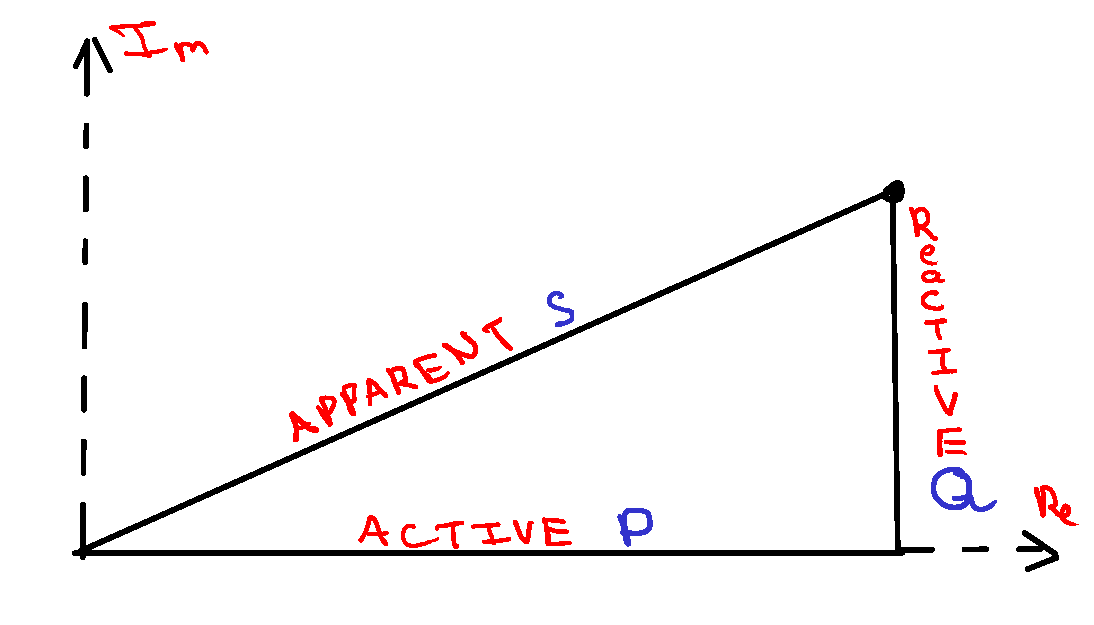
\includegraphics[width=0.6\textwidth]{xfigs/beer/beer.pdf}}
		\begin{tabular}{|cccc|}
			\hline
			\bf Name & \bf Type & \bf Symbol & \bf Unit \\\hline
			Complex Power & Complex Value & $S$ & VA \\
			Active Power & $ \text{Re}(S) $  & $P$ & W \\
			Reactive Power & $ \text{Im}(S) $  & $Q$ & VAr \\
			Apparent Power & $ |S| $  & $ |S| $  & VA \\
			\hline
		\end{tabular}
\end{center}

\subsection{Factors}
\begin{center}
	\begin{tabular}{rl}
		Power Factor &
		$ \cfrac{\text{Active Power}}{\text{Apparent Power}} = \text{Distortion Factor} * \text{Displacement Factor}$ \\
		Distortion Factor &
		$ \cfrac{\text{RMS of fundamental}}{\text{RMS of total}} = 1 \quad \text{(when no harmonics)} $ \\
		Displacement Factor &
		$ \cos \phi $, where $\phi$ is phase difference between voltage and current \\
	\end{tabular}
\end{center}
		
\section{Three-phase}
\begin{center}
		\begin{tabular}{|lcc|}
			\hline
			\bf Property & \bf Y & $ \pmb \Delta $ \\\hline
			Voltage&
			$ V_{LL} = \sqrt{3}V_\phi $ & 
			$ V_{LL} = V_\phi $ \\
			Current&
			$ I_L = I_\phi $ &
			$ I_L = \sqrt{3} I_\phi $ \\
			Phase&
			$ V_{ab} $ leads $ V_a $ by $30 ^\circ $ &
			$ I_{a} $ lags $ I_{ab} $ by $30 ^\circ $ \\
			Active Power &
			\multicolumn{2}{c|}{
				$ P = \sqrt{3}V_{LL}I_L \cos \phi $
			} \\
			Reactive Power &
			\multicolumn{2}{c|}{
				$ Q = \sqrt{3}V_{LL}I_L \sin \phi $
			} \\
			Apparent Power &
			\multicolumn{2}{c|}{
				$ |S| = \sqrt{3}V_\phi I_\phi $
			} \\
			\hline
		\end{tabular}
		\begin{itemize}
			\item All powers are given as total power
				( $ 3 * \text{Power of single load/coil}  $ )
			\item
				$ V_\phi $ is voltage across one coil.
			\item
				$ I_\phi $ is current through one coil.
			\item 
				$ \phi $  is phase difference between voltage and current
			(conventionally, voltage has 0 phase offset).
		\end{itemize}
\end{center}

\section{Magnetic Concepts}
\begin{center}
	\begin{tabular}{cccc}
		Field Strength & Flux Density & Magnetic Flux & Flux Linkage \\
		$H$ & $\vec{B}$ & $\Phi$ & $\lambda$ \\
		$[\unit{\ampere\per\meter}]$ &
		$[\unit{\tesla}] = [\unit{\volt\second\per\meter\squared}]$ &
		$[\unit{\weber}]$ &
		$[\unit{\weber}]$ \\
		- &
		$B = \mu_0 \mu_r H$ &
		$ \Phi = \vec{B} \cdot \vec{A}  $ &
		$ \lambda = N \Phi $ \\
		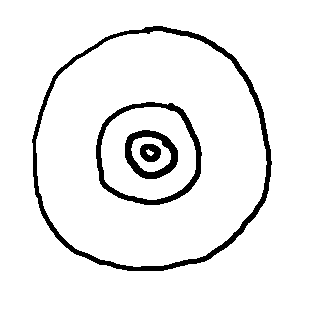
\includegraphics[width=0.15\textwidth]{xfigs/strength/strength.pdf} &
		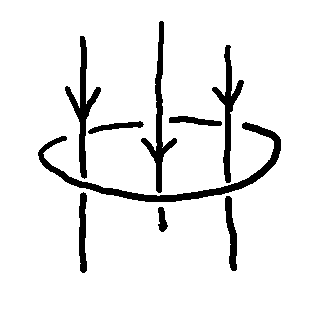
\includegraphics[width=0.15\textwidth]{xfigs/density/density.pdf} &
		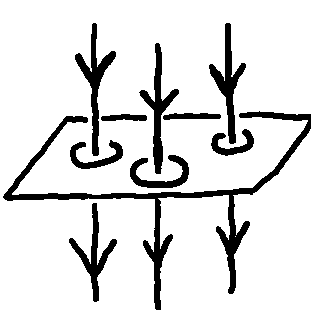
\includegraphics[width=0.15\textwidth]{xfigs/flux/flux.pdf} &
		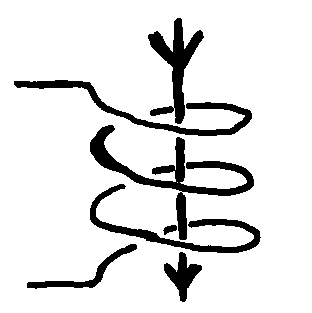
\includegraphics[width=0.15\textwidth]{xfigs/linkage/linkage.pdf} &
	\end{tabular}
\end{center}


\section{General Equations}
\begin{longtable}{lll}
	\makecell[l]
	{
		Speed
	} &
	\makecell[l]
	{
		$ [\unit{\meter\per\second}] = \cfrac{5}{18} [\unit{\km\per\hour}] $ 
	} &
	\makecell[l]
		{
	} \\

	\makecell[l]
	{
		Angular Speed
	} &
	\makecell[l]
	{
		$ v = \omega R $ 
	} &
	\makecell[l]
		{
			R is radius,
			v is linear speed.
	} \\

	\makecell[l]
	{
		Revolutions per Minute } & \makecell[l]
	{
		$ 
		[\unit{\radian\per\second}] = \cfrac{2\pi}{60} [\text{rpm}] $ 
	} &
	\makecell[l]
		{
	} \\

	\makecell[l]
	{
		Power
	} & \makecell[l]
	{
		$ P_{\text{mech}} = T \omega $ 
	} &
	\makecell[l]
		{
	} \\

	\makecell[l]
	{
		Turns Ratio: Voltage
	} &
	\makecell[l]
	{
		$ \cfrac{V_1}{V_2} = \cfrac{N_1}{N_2}  $ 
	} &
	\makecell[l]
		{
	} \\

	\makecell[l]
	{
		Turns Ratio: Current
	} &
	\makecell[l]
	{
		$ \cfrac{i_1}{i_2} = \cfrac{N_2}{N_1}  $ 
	} &
	\makecell[l]
		{
	} \\

\end{longtable}

\section{Converters}

\begin{itemize}
	\item Glavanic isolation (flyback converter only) 
		isolates high-voltage from low-voltage, more safe.
	\item Higher duty cycle = higher efficiency
\end{itemize}

\begin{center}
	\begin{tabular}{cccc}
		Value & Symbol & Unit & Notes \\\hline
		Duty Cycle & D & - & $ 0 < D < 1 $ \\
	\end{tabular}
\end{center}

\subsection{Buck}

\begin{longtable}{lll}
	\makecell[l]
	{
		Duty Cycle
	} &
	\makecell[l]
	{
		$ \cfrac{V_c}{V_s} = D $ 
	} &
	\makecell[l]
		{
	} \\

	\makecell[l]
	{
		Current
	} &
	\makecell[l]
	{
		$ I_B = \cfrac{V_s (D - D^2}{2 L f_s}  $ 
	} &
	\makecell[l]
		{
	} \\

\end{longtable}

\begin{itemize}
	\item Peak diode current = peak inductor current
	\item Peak inductor current = average inductor current * 2
\end{itemize}

\subsection{Flyback}

\begin{longtable}{lll}
	\makecell[l]
	{
		Duty Cycle
	} &
	\makecell[l]
	{
		$ \cfrac{V_c}{V_s} = \cfrac{N_2}{N_1} \, \cfrac{D}{1-D} $ 
	} &
	\makecell[l]
		{
	} \\

\end{longtable}



\section{DC Machines}
\begin{center}
	\begin{tabular}{cccc}
		Value & Symbol & Unit & Notes \\\hline
		Machine Constant & $K_m$ & ??? & Determined by geometry \\
		Field Constant & $K_\phi$ & ??? & Determined by geometry \\
		Pole Field & $ \phi_p $ & \unit{\weber} & - \\
		Torque & $ T $ & \unit{\newton\meter} & - \\
		Induced Voltage & $ e $ & \unit{\volt} & - \\
		Armature Voltage & $ r_a $ & \unit{\volt} & - \\
	\end{tabular}
\end{center}

\begin{longtable}{lll}
	\makecell[l]
	{
		Induced Voltage
	} &
	\makecell[l]
	{
		$ e = K_m \phi_p \omega $ 
	} &
	\makecell[l]
		{
	} \\

	\makecell[l]
	{
		Torque
	} &
	\makecell[l]
	{
		$ T = K_m \phi_p i_a $ 
	} &
	\makecell[l]
		{
	} \\

	\makecell[l]
	{
		Field per pole \\
		from Field Winding
	} &
	\makecell[l]
	{
		$ \phi_P = K_\phi i_f $ 
	} &
	\makecell[l]
		{
	} \\
\end{longtable}

\begin{center}
	\fbox{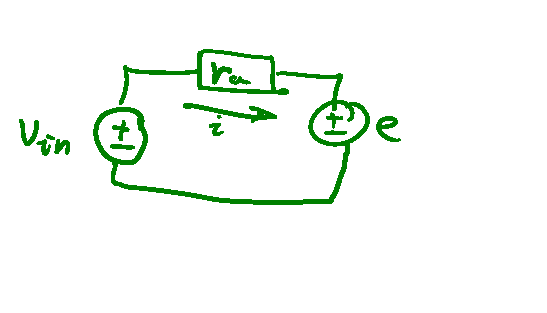
\includegraphics[width=0.8\textwidth]{xfigs/dc_machine/dc_machine.pdf}}
\end{center}



\section{AC Machines}
\begin{center}
	\begin{tabular}{cccc}
		Value & Symbol & Unit & Notes \\\hline
		Angular Speed & $n $ & rpm [revolutions per minute] & - \\
		Poles & $P$ & - & Always even \\
		Pole Pairs & $p$ & - & $p = \nicefrac{P}{2} $\\
		Slip & $s$ & ratio of angular speeds & $0 \leq s \leq 1 $ \\
	\end{tabular}
\end{center}

\begin{longtable}{lll}
	\makecell[l]
	{
		Synchronous Speed
	} &
	\makecell[l]
	{
		$ n_s [\text{rpm}]= \cfrac{120f [\unit{\hertz}]}{P} = \cfrac{60f [\unit{\hertz}]}{p}  $ 
	} &
	\makecell[l]
		{
	} \\

	\makecell[l]
	{
		Rotor Speed
	} &
	\makecell[l]
	{
		$ n_r = (1-s) n_s$
	} &
	\makecell[l]
		{
	} \\

	\makecell[l]
	{
		Synchronous Speed
	} &
	\makecell[l]
	{
		$ \omega_\text{mech} = \cfrac{2 \pi f_\text{elec}}{p}   $ 
	} &
	\makecell[l]
		{
	} \\

	\makecell[l]
	{
		Rotor Current Frequency
	} &
	\makecell[l]
	{
		$ f_r = s f_s $ 
	} &
	\makecell[l]
		{
	} \\

\end{longtable}

\begin{longtable}{lll}
	\makecell[l]
	{
		\meme Parama's equation
	} &
	\makecell[l]
	{
		$ P = \cfrac{V}{I}  $ 
	} &
	\textit{\makecell[l]
		{
			$V$ is voltage,
			$I$ is current,
			$P$ is power.
	}} \\
\end{longtable}

\end{document}

